\documentclass[article,a4paper]{IEEEtran}
\usepackage{lipsum}
\usepackage[backend=biber]{biblatex}
\usepackage{graphicx}

\addbibresource{refs.bib}
\title{Building Smarter Homes with IoT: Harnessing MQTT, Zigbee, and LoRa}
\author{
\IEEEauthorblockN{Anton Odén}\\
\IEEEauthorblockA{Dept. of Maths and Computer Science\\Karlstad University\\
651 88 KARLSTAD, Sweden}\\
anton.oden@outlook.com
}

\begin{document}

\maketitle

    \begin{abstract}
        
    \end{abstract}

    \section{Introduction}

    \section{Background}
    Communication in IoT is dependent on wireless communication, cause to connect all things by wire would quickly cover much of our space with wires and our wire-bill would match if not superseed the remaining infrastructure. Wireless communicaion could better be described as radio signals. Radio signals can be modulated to communicate at frequency, amplitud and phase and to avoid collision between different radio signals rules has been applied to what application could use what frequency. As radiosignals is used for defence capabilities there are hefty punishment \cite{RF-law} for transmitting in frequensies not sactioned by regional authority. Thought these rules could vary globally the ISM-bands different frequencies does has a globally ok coverage making it easier to produce communication hardware. For commercial usage different parts of the ISM-band has been opened/allowed to be used \cite{ISM-band1} and the most common commercial standard today in homes, offices, cafés etc. is IEEE 802.11, containing the commonly known WiFi protocol. Communicating at 2400-2483MHz (ISM-band), 5150-5350MHz, 5470-5725 (RLAN, EU standard EN 301 893) and newly introduced 5945-6425MHz (RLAN, EU standard EN 303 687) in WiFi 7 within Europe. \cite{ISM-bandEUR}. Starting from 2.4GHz in 1997 different frequencies bands has been added to satisfy our "desperate" need to high resolution video streaming. 
    \newline\newline
    One problem for IoT end devices that could be running on battery is that WiFi in its aim to give the user high data rate (bandwidth) is power consuming. WiFi is designed for high bandwidth that results in higher power consumption and for this reasons, new standards has been introduced to IEEE 802 family. 
    \newline\newline
    IEEE 802.15.4, which goes under the name Low-Rate Wireless Personal Area Network (LR-WPAN) is written with low power consumption in mind. The standard is grandfather of protocols such as Zigbee, 6LoWPAN, Thread, SNAP etc. Zigbee was first drafted 2004 and has became famous for usage in smart home implementations. It communicates at the 2400-2483MHz, which is same as WiFi. Also 868-868MHz in Europe and 902-928MHz in North America. Why the split between europe and north america may be Europe having more military applications communicating on 902-928MHz bandwidth \cite{ISM-bandEUR}. Getting the extra communication spectrums makes it easier for the protocol to communicate in highly density Wifi areas. 
    \begin{figure}
        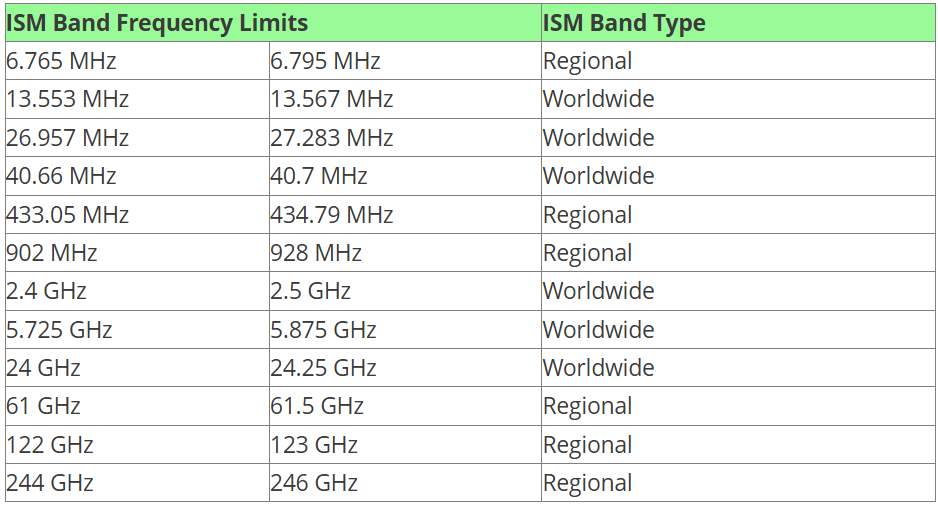
\includegraphics[width=\columnwidth]{ISM-band.png} 
        \caption{ISM-band frequency limits from \cite{ISM-band1}}
        \label{fig1:ISM-band frequency limits}   
    \end{figure}
    \ref{fig1:ISM-band frequency limits}
    Units within a zigbee network are categoriesed into three types. Coordinator, routers and end devices. The routers could be and often are an end device at the same time. The routers extend the physical range of the network and makes the network reliability as if one router goes offline the network so communication is not broken. This presupposes that end devices has more than one router in reachable range that can reach other parts of the network. The term mesh network is coined describing a zigbee network thought the network could also be structured in a star or tree topology also. "Mesh network: This is a network in which the routing of messages is performed as a decentrilized, cooperative proces involving many peer devices routing on each other's behalf." \cite{ZigbeeSpec}. So the routing devices are enabler of mesh network. The coordinator is only one within the personal area network and it is responsible of adding and decoupling devices to the network and the coordinator must be a fully functional device. End devices are all the things we want to connect in our IoT, usually a sensor/measuring instrument or some kind of actuator. 
    \newline\newline
    Another protocol in the LR-WPAN family is LoRaWAN which stand for Long Range Wide Area Network. It was developed for longer range communication. First of LoRa was developed for radiofrequency of 2-10km and then LoRaWAN was added on top to add network layer capabilities to the physical communication. LoRa radio frequency is divided between regions. Europe communicates 863-870MHz, USA 902-928MHz, China 470-510 and 779-787MHz etc. The division in the worlds LoRaWAN communication is illustraded in the fig3.
    \begin{figure}
        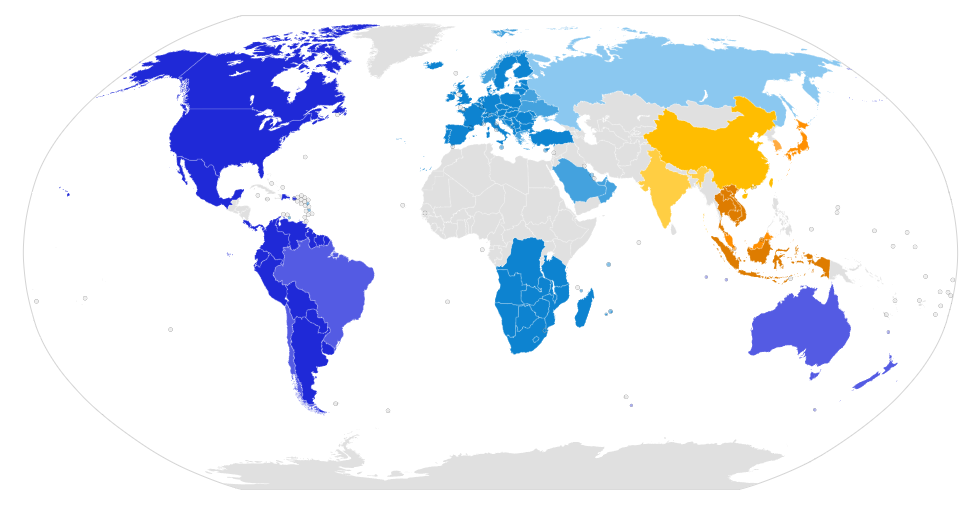
\includegraphics[width=\columnwidth]{LoRaWANdivide.png} 
        \caption{Map showing different frequencies in LoRa from \cite{LoRaWanfreqCountry}}
        \label{fig3:freq LoRaWAN}   
    \end{figure}
    \ref{fig3:freq LoRaWAN}
    LoRa transmit data with an technique called Chirp Spread Spectrum (CSS) that means that the transmitting is constantly modulates frequency \cite{LoraWanSpecOverview,LoRaTutorial}. For example Europes designated LoRa bandwidth 863-870MHz is further divided into allowed tranmission channels (regional channel plan) for uplink and downlink. One of those uplinks channels are 125kHz around 868,3MHz. Within that channel a transmission of bits is done by constantly modulating the frequency from lowest point 868,225MHz to channels highest point 868,375MHz (Eg. One chirp). Depending on what starting point within the chirp a specific symbol is being transmitted. A new tranmission allways starts with a set number of upchirps followed by some downchirps, letting the reciever know a datatransmission is starting. Transmission shifts between the allowed transmissionchannels in a pseudo-radom fashion. These frequency modulation and transmission shifting makes LoRa very resiliant to other transmission within the same bandwidth as the reciever can ignore other senders signals at noise as their current chirp status is with low propability the same and as LoRa is having a very far range capabilites alot of noise will be present.      
    \newline\newline
    To add functionality to the network another protocol is needed on top of network protocols, for example Zigbee or LoRaWAN that is used for the communication. The most famous protocol for this is Message Queue Telemetry Transport (MQTT) \cite{mqtt3.1.1,mqtt5.0}. MQTT filters all messages in a publish/subscribe manor. So MQTT terminology divide the network up in MQTT server/broker and MQTT clients, where the MQTT server is the central hub in the messaging system. All clients connected to the server published messages to the server, all published messages are labeled with a topic (usally friendly devicename for sensor IoT devices). All clients in the MQTT network can subscribe to specified published topics. So for example if an IRsensor send/publish a message with topic "AwesomeRobotSolutionIRSensor", all clients that are subscribing to topic "AwesomeRobotSolutionIRSensor" will recieve the published message via the MQTT broker. The MQTT header is designed to be lightweight which is convinient for IoT devices with low power consumption. The most basic ping message is reduced to only 2 bytes. To compare ICMP (Internet Control Message Protocol) requeries 8bytes header + 20 bytes IP header for a ping request \cite{ICMPping}. MQTT with it's 2bytes + zigbee network header of 8 bytes is 18 bytes or 2.8 times less in size. These reduction in packet sizes of the IoT protocols is what makes the low power consumption possible.
    \newline\newline
    A feature in MQTT is Quality of Service (QoS). In MQTT is is divided into 3 different cases \cite{mqtt3.1.1,mqtt5.0}. Both subsribing and publishing links does has the QoS setting to them. It is up to the user to set how important the messages sent are. Overhead (power consumption) is raised with higher level quality of service:
    \begin{itemize}
        \item QoS 0: At most once delivery. Messages are published with no demand of acknowledge if they got to the reciever end. -> PUBLISH
        \item QoS 1: At least once delivery. Reciever ackknowledge recieved message to sender making sender dicard sent message from memory buffer. If now ackknowledge recieved by sender a the message is published again until an ackknowledge is recieved. Hence final reciever could recieve multiple publishing messages of same type. -> PUBLISH <- PUBACK (fig2)
        \item QoS 2: Exactly once delivery. Adds a second back and forward between reciever and sender so that reciever does not register and forward multiple messages of the same publishing source. -> PUBLISH <- PUBREC -> PUBREL <- PUBCOMP.  
    \end{itemize}
    \begin{figure}
        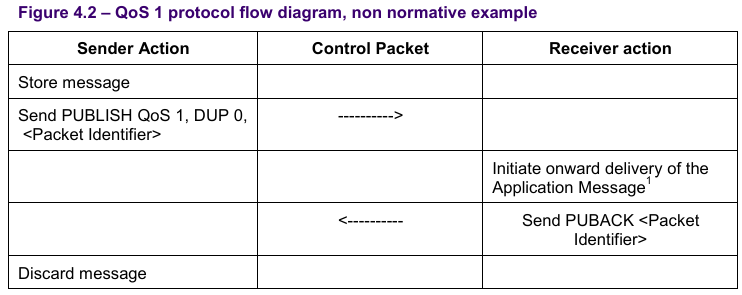
\includegraphics[width=\columnwidth]{QoS1.png} 
        \caption{QoS flow diagram from \cite{mqtt3.1.1}}
        \label{fig2:QoS1 flow diagram}   
    \end{figure}
    \ref{fig2:QoS1 flow diagram} 
    
    Topics in MQTT \cite{mqtt3.1.1} is structured with forward slashes to divide topics in a hierarchy with levels similar to folders and files in a file system.
    \begin{itemize}
        \item home/livingroom/temphum
        \item home/livingroom/lamp
    \end{itemize} 
    Knowing this a client can subscribe to all sensortypes with a single topic subscription using wildcards which could be stated to ignore different levels in the topic hierarchy. For example we can subsribe to all topics within our livingroom by subsribing to home/livingroom/\#. Or if we have lamps in other rooms in our home we could subsribe to home/+/lamp. As example shows we have + and \# sign to work with when using wildcards. There are more to talk about regarding MQTT but to finish with it is important to know that it's currently two versions of MQTT thats active today. MQTT 3.1.1 released in 2014 and MQTT 5.0 released in 2019. There a many examples on different protocols with MQTT alike features like MQTT-SN, ZeroMQ and AMQP that are worth mentioning thought MQTT is becoming industry standard. Some popular brokers/serversoftware using the MQTT protocol is Mosquitto, EMQX, VerneMQ, NanoMQ \cite{PopularMQTTprotocol}  There are also competing protocols to MQTT even if MQTT is becoming/already become industry standard.

    \section{The Challenges of Smart Home Networking}
    We have now went throught three different protocols. Two for communication (LoRaWAN and Zigbee) and another layor on top to be able to decide which device to transmitt to (MQTT). These are only a few of many different protocols and a challenge is to decide what protocol to use. Wifi has became synonymys with internet communication but as it's energy consumption is not suitable for battery powered units and another protocol is needed. One problem is that alot of different protocols are competeing in trying to be the protocol for battery driven smart home sensors. One movement to combine all these protocol in a overheadprotocol called Matter \cite{Matterspec} that is overseen by Connectivity Standards Alliance (former Zigbee Alliance). The specification is relative new with first revision released 2020 and it adds its main selling points is added IP-adresses and security.  The alliance was ,  Thread is developed One problem with Zigbee and LoRaWAN is that lacks IP-adresses. Thought cutting IP-adresses from the overhead in every transmission if saves battery power. 
    \section{Why Combine MQTT, Zigbee, and LoRaWan?}
    In a countryside home the area to cover often is bigger than in a a single house in the city. Alot of buildings outside and earthcellars for example could need more range capabilities that LoRaWAN can offer contra Zigbee. Also the buildings may lack electricity than further makes it harder to get in range with Zigbee as no routing devices can be added to the buildings. A homestead could have acres of land to collect data from where Zigbee lacks the nessisary length.  

    \section{Designing the Network Architecture}

    \section{Practical Use Cases}

    \section{Future Trends and Innovations}

    \section{Conclusion}

\printbibliography

\end{document}